% 2019-09-16
%
% Header can be about me and past tense: I have done X Y Z
%
% Body should describe results in the present tense, normal technical style
%
% The end of a section may use self-cites, and those may use past tense to
%  say "I did ...."

My research to date has focused on
 (1) understanding the performance challenges for natural~\cite{tfgnvf-popl-2016,gtnffvf-jfp-2019}
 and (2) analyzing the design space with novel theoretical foundations~\cite{gf-icfp-2018}.
These efforts have led up to the above thesis question.
The performance studies motivate a combination of \tdeep{} and \tshallow{}
 types and suggest methods to validate the result.
The design-space analysis provides a theoretical model for defining the
 combination and understanding its formal guarantees.

% This section reviews my prior work and explains how each project contributes
%  to the thesis question.


\subsection{Performance Evaluation}

Migratory typing promises the ability to mix typed and untyped code.
A performance evaluation for a migratory typing system must therefore
 evaluate mixed-typed programs.
My work proposed the first systematic evaluation method~\cite{tfgnvf-popl-2016},
 showed how to compare different implementations of migratory typing~\cite{gtnffvf-jfp-2019}
 and adapted the first method to programs with millions
 of ways to mix typed and untyped code~\cite{gm-pepm-2018,gtnffvf-jfp-2019}.

% Prior work did not measure mixed-typed programs~\cite{rsfbv-popl-2015,vss-popl-2017}.
% - rzv-ecoop-2015 do not measure code with runtime checks (sec 7.2, end)
% - aft-dls-2013 have mixed-typed variations of two benchmarks (sec 6.1)


\subsubsection{Summarizing Performance}

% NOTE
%The typical ``summary statistics'' of mean, median, min, and max were also a
% poor fit; although worst-case performance could be terrible
% (\figureref{fig:max-overhead}), there is no guarantee that a programmer
% will actually encounter the worst case.

%Turing's negative answer to the halting problem tells us that a computer
% program cannot tell the difference between an infinite running time and
% a very large one.

Our method of summarizing the performance in an exponentially-large set
 is based on a fundamental law of software development:
 all programs that are not ``fast enough'' are equally worthless.

\citet{tfgnvf-popl-2016} use this relevance law to summarize the performance
 of a migratory typing system.
If a configuration meets a fixed performance requirement, then it is good.
Otherwise it is worthless.
With this binary classification method, the performance of a mixed-typed
 program may be summarized by a single ratio; namely,
 the proportion of good configurations.
Likewise, a sequence of benchmarks may be summarized with a sequence of ratios.
These ratios can help software developers assess the performance risk of
 migratory typing.

Technically, a configuration is \deliverable{D}
 if its running time is no more than $D$x slower than the baseline performance
 with no migratory typing.\footnote{For example, in Racket, the fully-untyped configuration
 is an appropriate baseline. In transient Reticulated Python, the fully-untyped configuration
 run via Python (not via Reticulated) is an appropriate baseline because it is the starting
 point for a developer who wishes to migrate code~\cite{gm-pepm-2018}.}
Given a positive number $D$, the proportion of \deliverable{D} configurations
 is exactly the proportion of good configurations described above.

The paper accommodates varying notions of good performance by combining the
 results for $D$ between $1$ and $20$ into a plot.
The $x$-axis of such a plot ranges over values of $D$.
The $y$-axis ranges over the number (or percent) of configurations.
\Figureref{fig:snake-popl}, on the left-hand side, presents an example
 for a program with eight modules.
The key takeaway is that the plot answers an important question and does
 not require an exponential amount of space.

\begin{figure}[h]
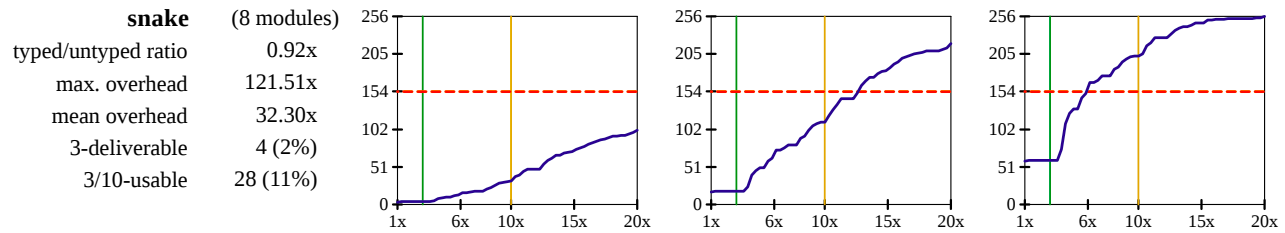
\includegraphics[width=0.96\columnwidth]{src/snake-popl.png}
\caption{Counting \deliverable{D} configurations in the \bm{snake}
         benchmark~\cite{tfgnvf-popl-2016}. The $x$-axis ranges over $D$ values;
         the vertical lines mark $D=3$ and $D=10$.
         The $y$-axis counts configurations; the dashed horizontal line marks
         $60$\% of all configs.
         The thick blue line is the number of \deliverable{x} configurations.}
\label{fig:snake-popl}
\end{figure}

Variations on the \deliverable{D} metric can answer similar questions
 about a mixed-typed program.
For example, the two other plots in \figureref{fig:snake-popl}
 relax the metric to allow 1 (middle plot) and 2 (right plot) extra type
 conversion steps.
In this case, one conclusion supported by the right-most plot is that
 if a $10$x slowdown is acceptable and the client is willing to add types
 to at most two extra modules, then 80\% of the configurations are within
 range of an acceptable state.
Once again the key takeaway is not the particular conclusion,
 but the fact that the method helps answer practical questions
 about the implementation of migratory typing.


\subsubsection{Comparing Implementations}
% Can the method compare different implementations of migratory typing?

The \deliverable{D} metric enables comparisons of different migratory
 typing systems.
If there are two languages that can execute the same program,
 then the language with better performance is the one that maximizes the
 proportion of \deliverable{D} configurations.

\citet{gtnffvf-jfp-2019} use this observation to compare three versions
 of Racket: v6.2, v6.3, and v6.4.
Racket~v6.3 contains a few improvements inspired by the performance
 evaluation of Racket v6.2~\cite{tfgnvf-popl-2016}.
Racket~v6.4 contains many more changes:
 it inlines the contract checks for simple typed functions,
 validates struct predicates with a first-order check,
 and reduces the memory overhead of contracts in general.
\Figureref{fig:snake-jfp} shows the effect of these changes on one benchmark.
The curve for version 6.4 lies above the others, meaning the percent of
 \deliverable{D} configurations is larger for every value of $D$ along
 the $x$ axis.

\begin{figure}[ht]
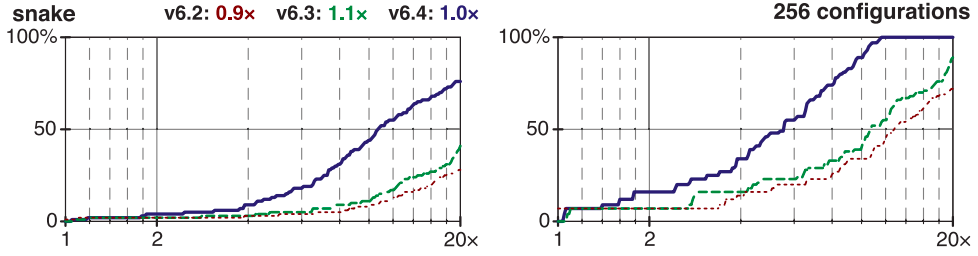
\includegraphics[width=0.8\columnwidth]{src/snake-jfp.png}
\caption{Comparing performance across three versions of Typed Racket; the right plot allows one type conversion step}
\label{fig:snake-jfp}
\end{figure}

Similar plots appear in related work:\footnote{\citet{kat-pldi-2019} plot the
 \deliverable{D} configurations in Typed Racket alongside a count based on
 the overhead of a new language, Grift, relative to Racket.
 The latter is not the \deliverable{D} metric because removing all typse from
 a Grift program does not produce a Racket program.}
\citet{bbst-oopsla-2017} demonstrate the benefits of adding a tracing JIT compiler to Typed Racket;
\citet{fgsfs-oopsla-2018} measure the impact of collapsible higher-order contracts; and
\citet{gf-icfp-2018} compare Typed Racket to a prototype implementation of transient type checks.


\subsubsection{Scaling the Method}
% Can the method be adapted to programs with a large number (+20) of configurations?

\citet{gm-pepm-2018} adapt the method to evaluate the performance of Reticulated
 Python.
In contrast to Typed Racket, Reticulated allows optional type annotations at
 a fine granularity.
Every function/method parameter, function return type, and class field may
 be optionally annotated.
Unfortunately for the exhaustive method, this freedom means that relatively
 small programs may have a huge number of configurations---counting
 the proportion of \deliverable{D} becomes impractical for a class with 20 fields.

The paper demonstrates, however, that a linear number of random samples can
 approximate the true number of good configurations.
Intuitively, the result says that the overhead experienced by $N$ developers
 provides useful information for the next one to add types to the same program.

To approximate the proportion of \deliverable{D} configurations,
 first select $s$ configurations uniformly at random and count the
 proportion of \deliverable{D} configurations in this sample.
Repeat for $r$ samples to build a set of proportions.
Use the set to build a confidence interval, and finally interpret the
 confidence interval to approximate the true proportion of deliverable configurations.

\citet{gm-pepm-2018} perform an experiment in which $r=10$ is a constant
 and $s = 10 * (F + C)$ is linear in the number of functions $F$ and classes
 $C$ in a benchmark.
For six benchmarks with 12 to 17 functions and classes each,
 they generate six 95\%~confidence intervals.
To validate these results, they collect the running time of every configuration
 in which: any function/method may be typed or untyped, and the set of fields
 for any class may be typed or untyped.
Note that this is fewer configurations than Reticulated allows.
% TODO more to say?
As \figureref{fig:sampling} shows, the confidence intervals provide a tight
 bound on the ground truth.

\begin{figure}[t]
  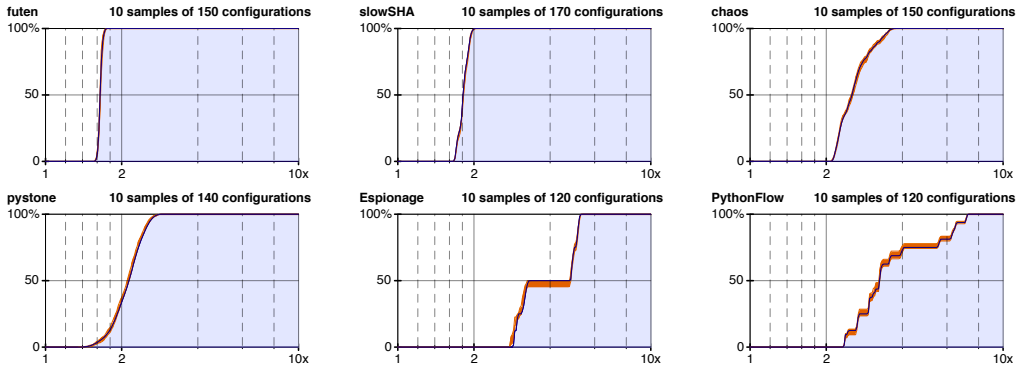
\includegraphics[width=\columnwidth]{src/sampling.png}
  \caption{Thin blue lines plot \deliverable{D} configurations; thick brown lines plot 95\% confidence intervals}
  \label{fig:sampling}
\end{figure}

\citet{gtnffvf-jfp-2019} validate this sampling method on Typed Racket
 programs.
They use the same number of samples and same linear sample size and find
 that the intervals yield tight approximations.

%Thanks to the approximation method, \cite{gm-pepm-2018} evaluate three programs
% with 19, 34, and 79 typed units each.


\subsubsection{Benchmark Suite}

\citet{gtnffvf-jfp-2019} formally introduce a suite of mixed-typed benchmark
 programs.
The benchmarks are available online\footnote{\shorturl{https://}{docs.racket-lang.org/gtp-benchmarks/}}
 and have been used to validate other changes to Typed Racket~\cite{gf-icfp-2018,bbst-oopsla-2017}.
% also Cameron (in submission) + Lukas (in submission)


\subsection{Design Space Analysis}

Models of migratory typing systems come in many varieties---often (but not always) because
 the models reflect a proof-of-concept implementation~\cite{bat-ecoop-2014,wnlov-popl-2010,mt-oopsla-2017,vss-popl-2017,tf-popl-2008,bat-ecoop-2014}.
 % TODO cite many more
These models share the common goal of mixing static and dynamic typing,
 but realize the goal with different formalizations.
Unfortunately, the diversity makes it difficult to compare properties of
 models in a scientific manner.

My work on comparing alternative approaches to migratory typing employs
 a model that expresses realizations as different semantics
 for a common surface language.
The common model enables well-founded comparisons of properties
 such as type soundness and complete monitoring.
Additionally, the model facilitates the design of new semantics for migratory
 typing.
% Need to mention other things? This paragraph should lead into the subsections


\subsubsection{A Spectrum of Type Soundness}

% developed model, (1) what are boundaries (2) what are checks
% implemented for TR
% - same method! aha
% - 

\citet{gf-icfp-2018} introduce a model to compare natural, erasure, and
 transient migratory typing as different semantics for a common surface
 language.
The common language is a mixed-typed system in the style of \citet{mf-toplas-2009};
 it syntactically combines a statically-typed language with a dynamically-typed
 language via boundary terms.
For example, the typed expression
 $(\eapp{(\edyn{(\tarr{\tint}{\tint})}{\efun{\svar_0}{\svar_0}})}{2})$
 applies a dynamically-typed value to a statically-typed input.
The type annotation $(\tarr{\tint}{\tint})$ helps the static type checker
 validate the application and may affect the behavior of a semantics.

In this model, the differences between type-enforcement strategies
 come about as different behaviors for boundary terms.
The natural semantics strictly enforces types at a dynamic-to-static
 boundary.
Incoming higher-order values get wrapped in a proxy to monitor their
 behavior; other values receive an exhaustive check (\figureref{fig:nt-boundary}, left).
At a static-to-dynamic boundary, the natural approach wraps outgoing
 higher-order values to protect against future untyped inputs.
Since higher-order values may appear within first-order data structures,
 the latter require a traversal.

The erasure semantics treats boundary terms as a no-op.
Any value may cross any boundary.

The transient semantics enforces boundary terms with tag checks (\figureref{fig:nt-boundary}, right);
 however, it also treats elimination forms in typed code as boundaries.
A dynamic-to-static boundary checks that the top-level shape of an incoming
 value matches the outermost constructor of the expected type.
A static-to-dynamic boundary lets any value cross; if typed code satisfies a
 tag-level soundness guarantee, then such values are certain to match the
 outermost constructor of the expected type.
Transient achieves this guarantee by guarding every elimination form in typed
 code with a dynamic-to-static check.
Thus if the untyped value $\epair{{-2}}{{0}}$ enters typed code via a
 $(\tpair{\tnat}{\tnat})$ boundary and typed code projects the first element
 of the pair expecting a nonnegative integer, a runtime check halts the program.

% note that checks overapproximate, but succeed without wrappers?

\begin{figure}[ht]
  \begin{minipage}[t]{0.5\columnwidth}
 \fbox{$\DNsym : \tpair{\stype}{\svalue} \rightarrow \svalue \cup \serror$}\\
  \(\begin{mfarray}
    \fDN{\tarr{\stype_0}{\stype_1}}{\svalue_0}
    & = &
    \emon{\tarr{\stype_0}{\stype_1}}{\svalue_0}
    \\\sidecond{if $\svalue_0$ is a function}
    \\
    \fDN{\tpair{\stype_0}{\stype_1}}{\epair{\svalue_0}{\svalue_1}}
    & = &
    \epair{\edyn{\stype_0}{\svalue_0}}{\edyn{\stype_1}{\svalue_1}}
    \\
    \fDN{\tint}{\sint_0}
    & = &
    \sint_0
    \\
    \fDN{\tnat}{\sint_0}
    & = &
    \sint_0
    \\\sidecond{if $0 \leq \sint_0$}
    \\
    \fDN{\stype_0}{\svalue_0}
    & = &
    \serror
    \\\sidecond{otherwise}
  \end{mfarray}\)

  \fbox{$\SNsym : \tpair{\stype}{\svalue} \rightarrow \svalue \cup \serror$}\\
  \(\begin{mfarray}
    \fSN{\tarr{\stype_0}{\stype_1}}{\svalue_0}
    & = &
    \emon{(\tarr{\stype_0}{\stype_1})}{\svalue_0}
    \\\sidecond{if $\svalue_0$ is a function}
    \\
    \fSN{\tpair{\stype_0}{\stype_1}}{\epair{\svalue_0}{\svalue_1}}
    & = &
    \epair{\esta{\stype_0}{\svalue_0}}{\esta{\stype_1}{\svalue_1}}
    \\
    \fSN{\stype_0}{\svalue_0}
    & = &
    \svalue_0
    \\\sidecond{otherwise}
  \end{mfarray}\)
  \end{minipage}\begin{minipage}[t]{0.5\columnwidth}
  \fbox{$\DTsym : \tpair{\stype}{\svalue} \rightarrow \svalue \cup \serror$}\\
  \(\begin{mfarray}
    \fDT{\tarr{\stype_0}{\stype_1}}{\svalue_0}
    & = &
    \svalue_0
    \\\sidecond{if $\svalue_0$ is a function}
    \\
    \fDT{\tpair{\stype_0}{\stype_1}}{\svalue_0}
    & = &
    \svalue_0
    \\\sidecond{if $\svalue_0$ is a pair}
    \\
    \fDT{\tint}{\sint_0}
    & = &
    \sint_0
    \\
    \fDT{\tnat}{\sint_0}
    & = &
    \sint_0
    \\\sidecond{if $0 \leq \sint_0$}
    \\
    \fDT{\stype_0}{\svalue_0}
    & = &
    \serror
    \\\sidecond{otherwise}
  \end{mfarray}\)

  \fbox{$\STsym : \tpair{\stype}{\svalue} \rightarrow \svalue \cup \serror$}\\
  \(\begin{mfarray}
    \fST{\stype_0}{\svalue_0}
    & = &
    \svalue_0
  \end{mfarray}\)
  \end{minipage}

  \caption{Boundary checks for natural (left) and transient (right)}
  \label{fig:nt-boundary}
\end{figure}

% ... spectrum of soundness
These three methods of enforcing type boundaries lead to three different
 semantics for surface programs.
One may compare the results of running one program via the three semantics,
 and one may formulate theorems that characterize general differences.
The models therefore serve as a tool for design analysis.
\citet{gf-icfp-2018} demonstrate this point by proving three pairs of type
 soundness theorems for the semantics.
For typed contexts, these theorems roughly guarantee the following:
 the natural semantics can only yield values that fully match the expected type;
 the erasure semantics can yield any value;
 and the transient semantics can only yield values with a tag that matches
 the outermost constructor of the expected type.
Sibling theorems describe the behavior of untyped code.

Additionally, the models serve as a tool for language design.
One may develop a new semantics by proposing a new strategy for checking
 the boundaries between typed and untyped components.
\citet{gf-icfp-2018} present two such variants of the natural semantics,
 dubbed co-natural and forgetful,
 that bridge the gap between natural and transient.
Co-natural allocates wrappers for all kinds of structured data---not only
 higher-order values---and thereby reduces the amount of checking at a boundary
 to a tag check.
Forgetful extends co-natural; if a wrapped value reaches a boundary, a new
 wrapper replaces the existing one.\footnote{The forgetful semantics and its
  type soundness are inspired by forgetful contracts~\cite{g-popl-2015}.}
Both co-natural and forgetful provide a type soundness guarantee that resembles
 type soundness for natural.
They both fail, however, to detect some type violations that natural detects.
Technically, co-natural detects more errors than forgetful, which detects
 more errors than transient~\cite{gf-icfp-2018}.


\subsubsection{A User Study}

\citet{tgpk-dls-2018} use the model of \citet{gf-icfp-2018} to create a survey about semantics
 for mixed-typed languages.
The survey employs the common surface syntax and three semantics:
 natural, erasure, and transient.
Each question presents one program and 2-3 possible outcomes of running
 the program.
Repondents must form an opinion based on two \emph{attitudes}:
 (1) do they like/dislike the behavior,
 and (2) do they find it expected/unexpected.
The two attitudes form a matrix of four possible answers.

The authors administered their survey to three populations:
 software engineers at a major Silicon Valley technology company;
 computer science students at a highly selective, private US university;
 and workers on Mechanical Turk who claimed to have programming experience.
They found a preference for the natural semantics---and more generally,
 for enforcing all claims implied by the types---across all three populations.


\subsubsection{Honest vs. Lying Types}

The different type soundness theorems for natural and transient
 demonstrate their different guarantees for typed code.
Clearly, natural-typed code can trust full types and transient-typed code
 can trust top-level type constructors.
Type soundness fails, however, to describe their different guarantees for
 untyped code.
Suppose that one untyped component $E$ expects a pair of numbers from a
 typed component;
 suppose further that the typed component provides a pair that it receives
 from a different untyped component---and that the pair contains strings
 rather than integers.

\[
  E[\esta{(\tpair{\tint}{\tint})}{(\edyn{(\tpair{\tint}{\tint})}{\epair{\estring{hello}}{\estring{world}}})}]
\]

\noindent
A natural semantics halts the program when the pair reaches the boundary to
 typed code.
A transient semantics lets the pair cross into typed code, and out to the
 untyped client.
Both behaviors are permitted by type soundness.
After all, soundness for untyped code has nothing to say about the type of a
 result value.
But the transient behavior means that untyped code cannot trust a typed
 API.

In general, a natural type is \emph{honest}\/ because it is a valid
 claim about all future behaviors of a value.
If natural accepts a value at a certain type, then it has either fully-checked
 the value or wrapped it in a monitoring proxy.
A transient type is valid in one specific context, and \emph{lying}\/
 to the rest of the program.
For example, the type $(\tpair{\tint}{\tint})$ above is only enforced in
 the visible typed component; the rest of the program cannot assume that the
 type is a valid claim about the contents of pairs that flow through the component.

\citet{gfd-oopsla-2019} formalize these intuitions with a complete
 monitoring theorem.
Complete monitoring comes from prior work on higher-order contracts;
 in brief, a contract system satisfies complete monitoring if every channel
 of communication between components is able to be monitored
 by a contract~\cite{dtf-esop-2012}.
A mixed-typed language satisfies complete monitoring if all communication
 across boundaries factors through runtime checks.
If so, then a pair value cannot smuggle a string such as $\estring{hello}$
 across a boundary that expects a number.

The key to proving a complete monitoring theorem is to enrich the syntax of
 the models with ownership annotations.
Ownership annotations state which components are responsible for the
 expressions and values in a program.
When a value flows across a boundary, its ownership changes depending on
 the type checks that occur.
If the checks fully validate the boundary type, the value replaces its previous
 owners with a new one.
Otherwise, the value keeps the previous owners and gains a new owner.
In this framework, a semantics satisfies complete monitoring iff it never
 lets a value accumulate more than one owner.
%A natural semantics satisfies complete monitoring and a transient
% semantics does not.

% note blame?



